% arara: xelatex: { shell: yes, synctex: yes }
%\RequirePackage[l2tabu, orthodox]{nag}
\documentclass[english,palatino]{ist-report}

\definecolor{bg}{rgb}{0.97,0.97,0.97}

% -- Bibliography
%\usepackage{csquotes}
%\usepackage{biblatex}
%\addbibresource{main.bib}

% -- Extra math options
\usepackage{mathtools}
\usepackage{siunitx} % Required for alignment
\sisetup{
  round-mode          = places, % Rounds numbers
  round-precision     = 2, % to 2 places
}

% -- Extra symbols
\usepackage{amssymb}
\usepackage{textcomp}
\usepackage{gensymb}
\usepackage{cancel}

% --  Image and float settings
\graphicspath{{graphics/}}
\usepackage{caption}
\usepackage{subcaption}
\usepackage{pdfpages}

% -- Graphs and diagrams
\usepackage{tikz}
\usepackage{pgfplots}
\usetikzlibrary{arrows.meta,positioning}
\pgfplotsset{compat=1.5, table/search path = {data}}

% -- Code listings
\usepackage{minted}
\setminted{linenos, bgcolor = bg, breaklines}
\setmintedinline{bgcolor = {}} 

% -- Extra table configs
\usepackage{booktabs}

\geometry{top=1.5cm}
\usepackage{todonotes}

\title{Integrated Avionic Systems}

\begin{document}

\thispagestyle{empty}

\begin{center}
	
\includegraphics[scale=0.3, trim = {93.4pt 219.7pt 77pt 221.9pt}]{IST_C_CMYK_POS}
	
	\vspace*{3mm}
	{\huge \textbf{Aircraft Altitude Control\\and Fault Processing}} \\
	\vspace*{4mm}
	{\large Control of an aircraft's altitude based on its sensor inputs and processing and mitigation of mid-flight system faults}
	\vspace*{4mm} \\
	\begin{tabular}{r l}
		Pedro \textsc{Afonso} & \textbf{66277} \\
		João \textsc{Manito} & \textbf{73096} \\
		Daniel \textsc{de Schiffart} & \textbf{81479}
	\end{tabular}
	
	\vspace*{3mm}
	{\Large \today}
	\vspace*{4mm} \\
	\rule{\linewidth}{0.5pt}
\end{center}

\begin{abstract}
	The objective of the second laboratory for this course was to control an aircraft's altitude and movement based on the input provided by its sensors and the transmission of data throughout the aircraft's onboard systems via its Local Area Network, characterizing the data protocols and preparing data for transmission. The second part of this laboratory had its focus more directed to the possibility of mid-flight faults to various aircraft systems, the handling of these faults and the simulation of data to maintain the control of the aircraft's altitude mentioned in the first part in the presence of faults in any of the crucial systems for this process. The work was to be implemented in MATLAB and its supporting software package \textit{Simulink}.
\end{abstract}

{\hypersetup{linkcolor = black} \tableofcontents}

\part{Aircraft Altitude Sensor and On-Board Data Bus}

This first part of the report focuses on the gathering of external data, in this case the pressure, through the on-board sensors, modelling of sensor behaviour using gathered data, and the comparison of this theoretical model with the actual data to study the error obtained. This work is followed by the study of the transmission of data through the aircraft's on-board system local network.

\section{Modeling The Input Data}

For this first section, we were provided a set of gathered voltage data from a sensor at three different temperatures, with each voltage value accompanied by the corresponding static pressure value. In total, a total of 219 lines of data, which means voltage values for 219 different real static pressure values. A sample of the data provided is seen in table \ref{tab:datain}.

\begin{table}[ht]
	\centering
	%\resizebox{\textwidth}{!}{
	\begin{tabular}{c|c|c|c}\toprule
		Pressure [mbar]		& Output [Volt] at $-45\degree C$	& Output [Volt] at $25\degree C$		& Output [Volt] at $125\degree C$	\\
		\midrule
		\num{1.0000000e+01}	& \num{9.6891912e-02}				& \num{3.9214138e-02}					& \num{8.0487284e-02}				\\
		$\vdots$			& $\vdots$							& $\vdots$								& $\vdots$							\\
		\bottomrule
	\end{tabular}
	%}
	\caption{Example of the provided data formatting.}
	\label{tab:datain}
\end{table}

The data was to be used to determine a model for the pressure, using the voltage and ambient temperature as model inputs. For this purpose, we used MATLAB's \href{https://www.mathworks.com/help/curvefit/fit.html}{\texttt{fit}} function from the \textit{Curve Fitting Toolbox}, using a second order polynomial for the temperature axis and a fourth-order polynomial curve for the voltage fitting. This yielded the polynomials found in equation \ref{eq:fitpoly}.

\begin{gather}\label{eq:fitpoly}
	%p(v,T) = 27.21 + 311.6v + 0.05789T - 20.33v^2 + 0.1015vT
	\begin{split}
		p(v,T) = 5.639 + 382.1v - 0.05732T - 69.73v^2 + 0.2646vT + 0.0002634T^2 + 11.53v^3 \\ - 0.05126v^2T - 0.0002063vT^2 - 0.8314v^4 + 0.004329v^3T + 4.644\times10^{-5}v^2T^2
	\end{split}
\end{gather}

The model was plotted against the provided input data and can be found in figure \ref{fig:3dplotmain} in page \pageref{fig:3dplotmain}.
%The raw data from the MATLAB output can be found below.  
%
%\begin{minted}{text}
%Linear model Poly42:
%     sf(x,y) = p00 + p10*x + p01*y + p20*x^2 + p11*x*y + p02*y^2 + p30*x^3 + 
%                    p21*x^2*y + p12*x*y^2 + p40*x^4 + p31*x^3*y + p22*x^2*y^2
%     Coefficients (with 95% confidence bounds):
%       p00 =       5.639  (1.566, 9.713)
%       p10 =       382.1  (371.3, 392.9)
%       p01 =    -0.05732  (-0.1234, 0.008728)
%       p20 =      -69.73  (-78.75, -60.72)
%       p11 =      0.2646  (0.166, 0.3632)
%       p02 =   0.0002634  (-0.0003534, 0.0008803)
%       p30 =       11.53  (8.749, 14.31)
%       p21 =    -0.05126  (-0.0942, -0.008322)
%       p12 =  -0.0002063  (-0.0008547, 0.0004422)
%       p40 =     -0.8314  (-1.113, -0.5502)
%       p31 =    0.004329  (-0.001359, 0.01002)
%       p22 =   4.644e-05  (-8.942e-05, 0.0001823)
%\end{minted}

\section{Modelling of a temperature data ADC}
For this question we considered the range of values between $\num{-45}\degree C$ and $\num{125}\degree C$, which leaves us with a total of 170 values of temperature to be transmitted. With an additional request of an accuracy of $\num{0.1}\degree C$, we need ten times as many values. All things considered, we need to transmit any values in a range of 1700 possibilities. Going through the amount of possible values held by a number of binary bits, we look for the amount of bits to meet this requirement.

\begin{table}[ht]
	\centering
	\begin{tabular}{ccc}
		\vdots		& $=$	& \vdots	\\
		$2^9$		& $=$	& $512$		\\
		$2^{10}$	& $=$	& $1024$	\\
		$2^{11}$	& $=$	& $2048$	\\
		$2^{12}$	& $=$	& $4096$	\\
		\vdots		& $=$	& \vdots	\\
	\end{tabular}
\end{table}

With this in mind, and considering using an offset of values to eliminate the need for a signal bit (or even converting the temperature to Kelvin), we need at the very least 11 bits to transmit.

\section{Evaluation of model error and ADC accuracy in altitude determination}
In order to be able to feed the pressure sensor data to the Air Data Computer, a Analog to Digital conversion has to be performed. This in turn leads us to a question: how much resolution is needed for the conversion? Obviously, the minimum ammount of bits necessary must be able to go from 0 to the maximum value necessary. In this case, the ISA mean sea level altitude is defined by a pressure of 1013.25 mbar; As such, at least 10 bits (1024 steps) are necessary to contain the entire range of pressures from sea level to vaccum. However, since there are locations on the planet with pressure altitudes below ISA mean sea level, we decided to require at least 11 bits of resolution, to ensure those locations are correctly included. However, a more accurate pressure determination is required to ensure that pressure altimeter errors are small enough for this system to be used for air travel. For this effect, we defined that the ADC shall have a fixed point output, with 11 integer part bits and N fractional bits. To determine the number of fractional bits required, we created a set of pressure values, simulating the pressure range of the International Standard Atmosphere. 

Simulating a pressure sensor with an ADC, we determined the conversion altitude error. The results for N=3 (total 14 bits) and N=4 (total 15 bits) are presented in Figures \ref{fig:N3} and \ref{fig:N4}. As we can see, both present small errors, in the order of meters. Taking into account that we are working with modeled, ideal sensors, without noise and ignoring a plethora of other factors, we decided to go with N=4 (total 15 bits) as the operational requirement for the number of ADC bits. This allows us to have a larger tolerance for any problems that might arise in the use of the sensor, while still allowing meter-order errors in the altitude determination, enough to ensure a safe vertical separation between aircraft.
%By discretizing these values for each number of bits of the ADC conversion we intended to study and feeding these values to the pressure-voltage model obtained in Section 1 (see Figure \ref{fig:2dplotmain}) we obtained a set of voltages that model the sensor output to an increase of altitude in the ISA. We then computed the pressure returned by this sensor+ADC system using the model from \ref{eq:fitpoly}. In the end, we converted this pressure to pressure altitude and determined it's error relative to the true pressure altitude, calculated using the set of initial pressure values. The results for N=3 (total 14 bits) and N=4 (total 15 bits) are presented in Figures \ref{fig:N3} and \ref{fig:N4}. As we can see, both present small errors, in the order of meters. Taking into account that we are working with modeled, ideal sensors, without noise and ignoring a plethora of other factors, we decided to go with N=4 (total 15 bits) as the operational requirement for the number of ADC bits. This allows us to have a larger tolerance for any problems that might arise in the use of the sensor, while still allowing meter-order errors in the altitude determination, enough to ensure a safe vertical separation between aircraft.

\begin{figure}
	\centering
	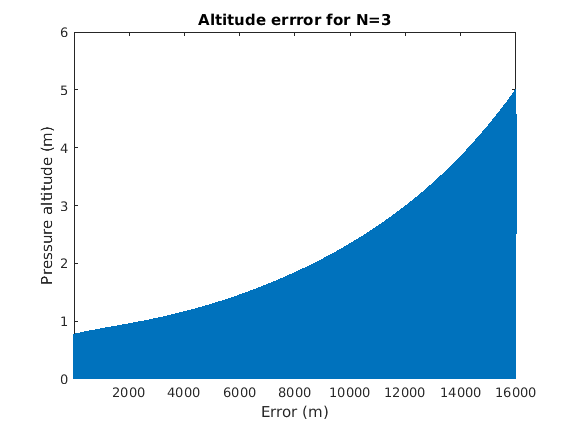
\includegraphics[width=0.6\textwidth]{graphics/N3.png}
	\caption{Simulation result error for N=3}
	\label{fig:N3}
\end{figure}


\begin{figure}
	\centering
	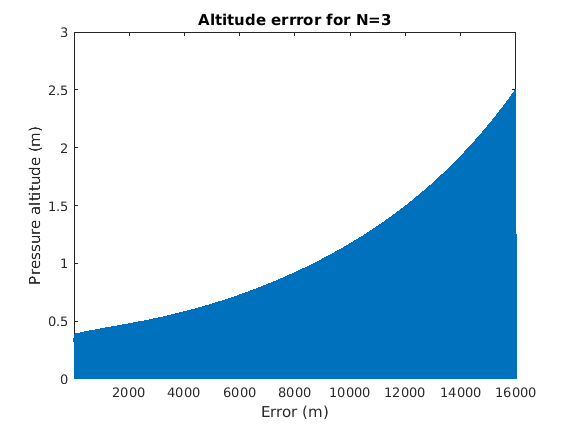
\includegraphics[width=0.6\textwidth]{graphics/N4.png}
	\caption{Simulation result error for N=4}
	\label{fig:N4}
\end{figure}


\section{ARINC 429 Data Bus Sketching}
The ARINC 429 Data Bus that was designed in order to provide the Air Data Computer with the needed inputs is presented in Figure \ref{fig:adc}.


\begin{figure}[ht]
	\centering
	%\resizebox{\textwidth}{!}{
	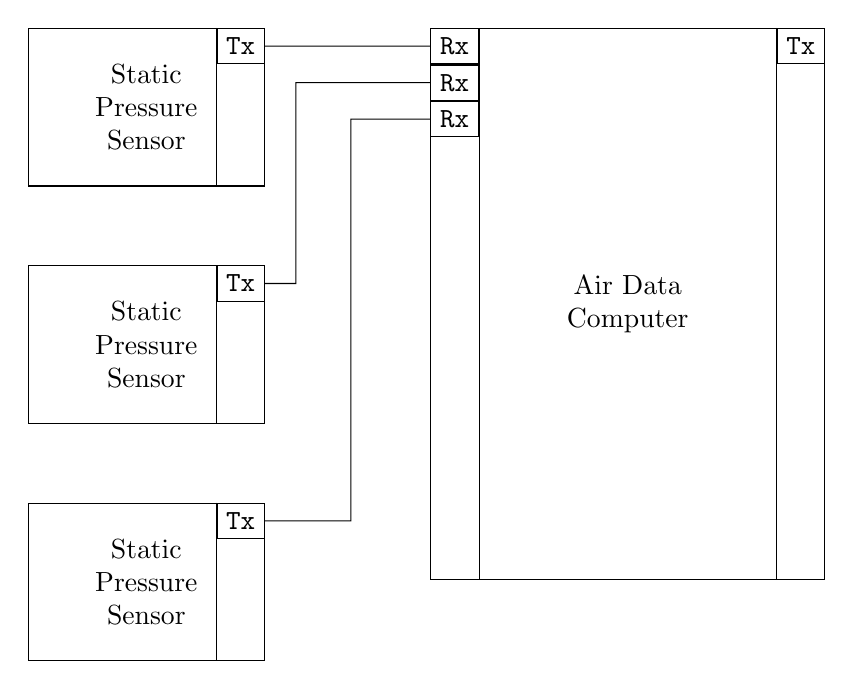
\begin{tikzpicture}[scale=0.7]
		\node (sp1) at (0,0) [rectangle, draw, align=center,minimum width = 3cm, minimum height = 2cm] {Static \\ Pressure \\ Sensor};
		\node (tx11) at (sp1.north east) [rectangle,draw,anchor = north east] {\texttt{Tx}};
		\path [draw,very thin] (tx11.north west) -- (tx11.north west|-sp1.south);
		\node (sp2) [below=of sp1,rectangle, draw, align=center,minimum width = 3cm, minimum height = 2cm] {Static \\ Pressure \\ Sensor};
		\node (tx21) at (sp2.north east) [rectangle,draw,anchor = north east] {\texttt{Tx}};
		\path [draw,very thin] (tx21.north west) -- (tx21.north west|-sp2.south);
		\node (sp3) [below=of sp2,rectangle, draw, align=center,minimum width = 3cm, minimum height = 2cm] {Static \\ Pressure \\ Sensor};
		\node (tx31) at (sp3.north east) [rectangle,draw,anchor = north east] {\texttt{Tx}};
		\path [draw,very thin] (tx31.north west) -- (tx31.north west|-sp3.south);
		\path (sp1.north east) ++(3,0) node (adc) [anchor = north west, rectangle, draw, align=center, minimum width = 5cm, minimum height = 7cm] {Air Data \\ Computer};
		\node (rxa1) at (adc.north west) [rectangle,draw,anchor = north west] {\texttt{Rx}};
		\path [draw,very thin] (rxa1.north east) -- (rxa1.north east|-adc.south);
		\node (rxa2) at (rxa1.south west) [rectangle,draw,anchor = north west] {\texttt{Rx}};
		\node (rxa3) at (rxa2.south west) [rectangle,draw,anchor = north west] {\texttt{Rx}};
		\node (txa1) at (adc.north east) [rectangle,draw,anchor = north east] {\texttt{Tx}};
		\path [draw,very thin] (txa1.north west) -- (txa1.north west|-adc.south);
		\path [draw] (tx11) -- (rxa1);
		\path [draw] (tx21)  -- ++(1,0) coordinate (c1) -- (c1|-rxa2) -- (rxa2);
		\path [draw] (tx31)  -- ++(2,0) coordinate (c2) -- (c2|-rxa3) -- (rxa3);
	\end{tikzpicture}
	%}
	\caption{Air Data Computer.}
	\label{fig:adc}
\end{figure}

\begin{gather*}
	h(p) = 145366.45\left(1 - \left(\frac{p_s}{1013.25}\right)^{0.190284}\right)
\end{gather*}

\part{Dealing With Faults and Errors}

For this section of the laboratory project the focus was to analyze and test possible faults within the components of the system and study and implement methods to deal with these problems. For this very purpose, we needed to design a simple aircraft controller and perform any tests and implementations around it.

\section{Modelling The Aircraft's Motion}\label{sec:plant}

Per request of the teacher, the objective was to use a simplified model of an aircraft and its behaviour and design and implement an altitude controller. The considered plant variables were the horizontal position $x$, the altitude $h$, the horizontal and vertical velocities (or rate of change of both previous variables) $\dot{x}$ and $\dot{h}$, and the flight path angle $\gamma$. Also per request, the variables to be controlled were the angle of attack $\alpha$ and the engine power, which we took the liberty of changing to the engine thrust $T$ as a variable of force. The variables were all considered in their correspondent SI units.

The variables and their corresponding units and initial considered values can be found in table \ref{tab:controllervars}.
\begin{table}[ht]
	\centering
	\begin{tabular}{c|c|c|c}\toprule
		Variable		& Description			& Unit						& Initial Values	\\
		\midrule
		$x$				& Horizontal position	& \si{\meter}				& $0$				\\
		$h$				& Altitude				& \si{\meter}				& $0$				\\
		$\dot{x}$		& Horizontal speed		& \si{\meter\per\second}	& $65.8354$		   	\\
		$\dot{h}$		& Altitude rate			& \si{\meter\per\second}	& $0$				\\
		$\gamma$		& Flight path angle		& $rad$     				& $0$			    \\
		$\alpha$		& Angle of attack		& $rad$		        		& $0.052534$		\\
		$T$             & Thrust force          & \si{\newton}              & $500$                \\
		\bottomrule
	\end{tabular}
	\caption{The variables used in the description of the aircraft behaviour and their respective units.}
	\label{tab:controllervars}
\end{table}

\begin{figure}
	\centering
	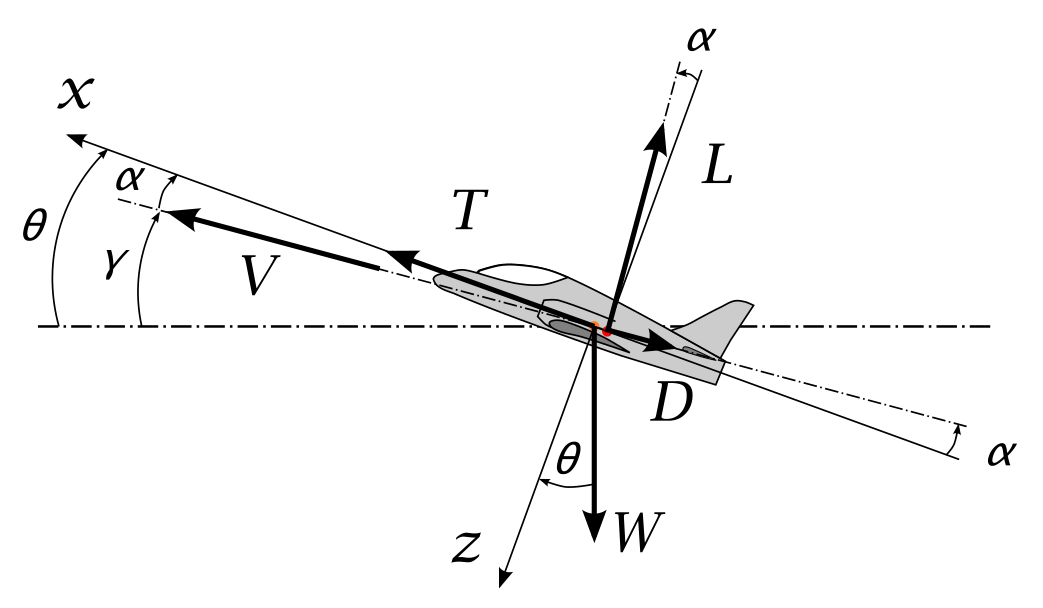
\includegraphics[width=0.6\textwidth]{aircraft}
	\caption{Aircraft body referential and relevant angles used in the description of the aircraft behaviour.}
	\label{fig:bodyref}
\end{figure}

The dynamic equations were derived from standard aircraft behaviour obtained from other relevant literature. Using the relations found in figure \ref{fig:bodyref}, we derived the equations for the basic horizontal movement and altitude rates that can be found in equations \ref{eq:x_rate} and \ref{eq:h_rate}.
\begin{align}\label{eq:x_rate}
	\frac{dh}{dt} &= V(t)\sin{\gamma(t)} \\
	\label{eq:h_rate}
	\frac{dx}{dt} &= V(t)\cos{\gamma(t)}
\end{align}
Within these equations we see the first appearance of the $V$ variable, which we will use for the scalar velocity of the aircraft as the Pythagorean sum of both rates of movement referenced in table \ref{tab:controllervars}.

Redirecting our attention back to figure \ref{fig:bodyref} we can obtain a value for the resultant force of the aircraft by considering all the forces acting on it in every moment. By considering all the forces in the direction of the movement, using Newton's first law $\mathbf{F} = m\mathbf{a}$, and considering $a = \dot{v}$, we can write down the rate of the aircraft's aforementioned scalar velocity.
\begin{gather}\label{eq:v_rate}
	m\dot{V} = m\frac{dV(t)}{dt} = T - D - mg\sin\gamma
\end{gather}
Rounding all that up, together with an equation for the rate of change of the flight path angle $\dot{\gamma}$, we obtain the reference equations \ref{eq:v_rate_main} and \ref{eq:gamma_rate}.
\begin{align}
	\label{eq:v_rate_main}
	\frac{dV(t)}{dt} = \dot{V} &= \frac{1}{m}\left(T - D - mg\sin\gamma\right) \\
	\label{eq:gamma_rate}
	\frac{d\gamma}{dt} \dot{\gamma} &= \frac{1}{mv}\left(L - mg\cos\gamma\right)
\end{align}
Further simplifications were taken into account to raise expedience for the controller design and facilitate its implementation. Since we want to focus on the aircraft and the on-board system's behaviour and response to faults and errors, we could assume that the initial undisturbed condition would be stable level flight. This means we can consider the rates of altitude, horizontal velocity and flight path angle to be zero. So,
\begin{gather*}
	\dot{h} = \dot{x} = \dot{\gamma} = 0
\end{gather*}
This meant that some components in equations \ref{eq:v_rate_main} and \ref{eq:gamma_rate} could be cut, which leaves us with equations \ref{eq:h_rate_simp}, \ref{eq:v_rate_simp} and \ref{eq:gamma_rate_simp}.
\begin{align}
	\label{eq:h_rate_simp}
	\dot{h} = V\sin\gamma = 0 &\Rightarrow \left\{\begin{aligned}
		&\cancel{V = 0} \\
		&\sin\gamma = 0 \Rightarrow \gamma = 0 \vee \cancel{\gamma = \pi}
	\end{aligned}\right. \\
	\label{eq:v_rate_simp}
	\dot{v} = 0 &\Rightarrow 0 = \frac{1}{m}\left(T - D - mg\right) \Rightarrow T = D + mg \\
	\label{eq:gamma_rate_simp}
	\dot{\gamma} = 0 &\Rightarrow 0 = \frac{1}{mv}\left(L - mg\right) \Rightarrow L = mg
\end{align}
On the first equation above (\ref{eq:h_rate_simp}) we can assume the null value for $\gamma$ as the other values obtained from the equation have no physical meaning in this simulation.

The aircraft aerodynamic forces for lift and drag can be decomposed into their adimensional equivalents, for which data can be obtained from analogous sources without many adjustments. This way, we can obtain the values for these forces based on current flight status.
\begin{align}
	\label{eq:cd} C_D = \frac{D}{\frac{1}{2}\rho V^2S} &\Rightarrow D = \frac{1}{2}\rho V^2SC_D \\
	\label{eq:cl} C_L = \frac{L}{\frac{1}{2}\rho V^2S} &\Rightarrow L = \frac{1}{2}\rho V^2SC_L
\end{align}
Applying this logic to the previous equations we can replace the absolute values of forces with adimensional data.
\begin{gather*}
	T\cos\alpha = D \Rightarrow T_0\cos{\alpha_0} = \frac{C_D\rho V_0^2S}{2} \\
	T\sin\alpha + L = mg \Rightarrow T_0\sin{\alpha_0} + \frac{C_L\rho V_0^2S}{2} = mg
\end{gather*}

\section{The Controller}

To implement the controller we had to define the inputs and their relations with the outputs and the aircraft dynamics, which were mentioned and described in section \ref{sec:plant}.

For this reason, we define the aircraft's states as the vector $\mathbf{x}$ and the aircraft's inputs as vector $\mathbf{u}$, where a bold typeface represents a non-scalar variable, lowercase for vectors and uppercase for matrices.
\begin{gather*}
	\mathbf{x} = \left[\begin{matrix}h & v & \gamma\end{matrix}\right]^T \qquad \mathbf{u} = \left[\begin{matrix}\alpha & T\end{matrix}\right]^T
\end{gather*}
With this notation we can define the aircraft's behaviour as defined below.
\begin{gather*}
	\dot{\mathbf{x}} = \mathbf{A}\mathbf{x} + \mathbf{B}\mathbf{u}
\end{gather*}
Both the matrices referenced here can be defined by the aforementioned variables and inputs.
\begin{gather*}
	\mathbf{A} = \left[\begin{matrix}
			\frac{\partial\dot{h}}{\partial h}		& \frac{\partial\dot{h}}{\partial v}		& \frac{\partial\dot{h}}{\partial \gamma} \\
			\frac{\partial\dot{v}}{\partial h}		& \frac{\partial\dot{v}}{\partial v}		& \frac{\partial\dot{v}}{\partial \gamma} \\
			\frac{\partial\dot{\gamma}}{\partial h}	& \frac{\partial\dot{\gamma}}{\partial v}	& \frac{\partial\dot{\gamma}}{\partial \gamma}
		\end{matrix}\right]
		\qquad \mathbf{B} = \left[\begin{matrix}
			\frac{\partial\dot{h}}{\partial \gamma}			& \frac{\partial\dot{h}}{\partial T}		\\
			\frac{\partial\dot{v}}{\partial \gamma}			& \frac{\partial\dot{v}}{\partial T}		\\
			\frac{\partial\dot{\gamma}}{\partial \gamma}	& \frac{\partial\dot{\gamma}}{\partial T}
		\end{matrix}\right]
\end{gather*}
Referring to the equations \ref{eq:h_rate_simp}, \ref{eq:v_rate_simp} and \ref{eq:gamma_rate_simp}, we can write down the matrices with the corresponding derivatives applied, simplified to depend only on the control and input variables (making use of the simplifications on equations \ref{eq:h_rate_simp}, \ref{eq:v_rate_simp} and \ref{eq:gamma_rate_simp}, and using the coefficients in equations \ref{eq:cd} and \ref{eq:cl}).
\begin{gather}
	\label{eq:a_matrix}
	\mathbf{A} = \left[\begin{matrix}
			0	& \sin\gamma_0				& V_0\cos\gamma_0								\\
			0	& -\frac{C_D\rho V_0S}{m}	& -g\cos\gamma_0								\\
			0	& \square					& \frac{g\sin\gamma_0}{V_0}
		\end{matrix}\right],
		\quad
		\square = -\frac{T_0\sin\alpha_0}{mV^2} + \frac{C_L\rho S}{2m} + \frac{g\cos\gamma_0}{V_0^2} \\
	\label{eq:b_matrix}
	\mathbf{B} = \left[\begin{matrix}
			0								& 0							\\
			-\frac{T_0\sin\alpha_0}{m}		& \frac{\cos\alpha_0}{m}	\\
			\frac{T_0\cos\alpha_0}{mV_0}	& \frac{\sin\alpha_0}{mV_0}
		\end{matrix}\right]
\end{gather}
Finally, we get the state-space equation in short form.
\begin{gather}\label{eq:statespace}
	\left[\begin{matrix} \dot{h} \\ \dot{V} \\ \dot{\gamma} \end{matrix}\right] = \mathbf{A}\left[\begin{matrix} h \\ V \\ \gamma \end{matrix}\right] + \mathbf{B}\left[\begin{matrix} \alpha \\ T \end{matrix}\right]
\end{gather}


Constant values from airplane:
\begin{gather*}
C_l = 0.476 \qquad
C_d = 0.016 \qquad
m = \SI{1518.44}{\kilogram} \qquad
\rho (\textrm{Air density}) = \SI{1.2}{\kilogram\per\meter\cubed} \\
S (\textrm{Wing Area}) = \SI{12}{\meter\squared} \qquad
g (\textrm{Gravity acceleration}) = \SI{9.8}{\meter\per\second\squared} \\
T_0 (\textrm{Thrust in equilibrium}) = \SI{500}{\newton}
\end{gather*}

\begin{figure}
	\centering
	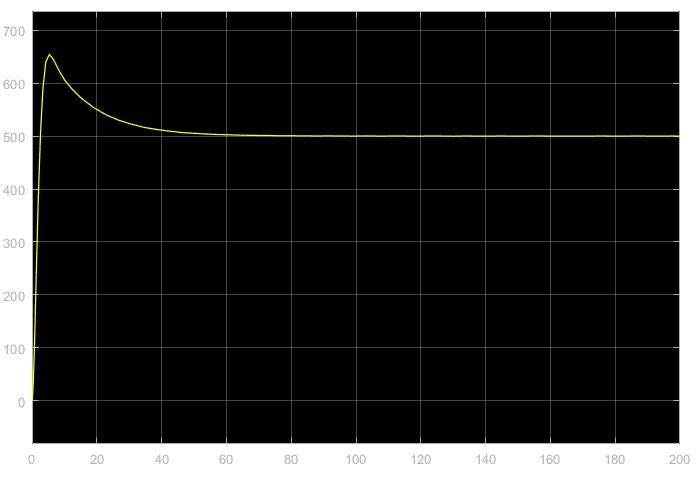
\includegraphics[width=0.6\textwidth]{graphics/hsim.jpg}
	\caption{Controller altitude simulation.}
	\label{fig:bodyref}
\end{figure}


\section{Possible Faults}

Within the simple system implemented in this laboratory, several components can fail or behave unexpectedly. Whether it's the control system or the sensors used, either one can have a fault at some point and the control system needs to be ready to return the control to the pilot should a fault be detected somewhere.

This fault detection will be done by monitoring the flight variables and their behaviour throughout the simulation. The first step should then be define what constitutes a fault. By definition,
\begin{quote} \itshape
	A fault is a deviation (of a feature) from the acceptable, standard operational condition.
\end{quote}
For sensors, we can consider four types of faults, either sensor bias, drift, loss of accuracy or freeze. The sources for these faults come from either the barometric sensor or the temperature A/D conversion. For the bus, we can consider physical loss of the bus and data corruption as our faults.

We then modeled a few failure modes for the controller. While at first glance some seem different from the faults above, the above faults can be considered subsets of these failure modes: signals above a given limit and signals that change too fast ("spikes"). Afterwards, we added these failure mode models to the simulator, ending with an architecture that is designed to detect errors and return the control of the aircraft to the pilot, emulated in this simulation with a simulation stop. We simulated a combination between every type of faults, injected manually, and for each situation in the presence of a fault the simulation was stopped and a control flag set to true corresponding to the failure. This represents the transfer of control to the pilot and simultaneous warning to the pilot of the presence of a fault and its origin. Since this analysis is "binary" in nature, there are no relevant plots to present.

\section{Architecture for a fault tolerant controller}

For the present lab work, we created a triplex architecture for fault tolerance. This architecture is present in the simulink file triplex.slx.



\pagebreak
\appendix

\section{Data Plots}

\begin{figure}[ht]
	\centering
	\begin{tikzpicture}
		\begin{axis}[domain=0:5,y domain=-45:125,view={-30}{25},xlabel=$\si{\volt}$,ylabel=$\degree C$, zlabel=$\si{\pascal}$,width=0.7\textwidth]
			\addplot3[surf,samples=5] {5.639 + 382.1 * x - 0.05732 * y - 69.73 * x^2 + 0.2646 * x * y + 0.0002634 * y^2 + 11.53 * x^3 - 0.05126 * x^2 * y - 0.0002063 * x * y^2 - 0.8314 * x^4 + 0.004329 * x^3 * y + 4.644 * 0.00001 * x^2 * y^2};
			\addplot3[only marks,color=red,mark=o] table [x index = {1}, z index = {0}, y expr = -45, col sep = comma] {inputdata.csv};
			\addplot3[only marks,color=blue,mark=o] table [x index = {2}, z index = {0}, y expr = 25, col sep = comma] {inputdata.csv};
			\addplot3[only marks,color=green,mark=o] table [x index = {3}, z index = {0}, y expr = 125, col sep = comma] {inputdata.csv};
		\end{axis}
	\end{tikzpicture}
	\caption{Comparison of the data provided and the modelled polynomial.}
	\label{fig:3dplotmain}
\end{figure}

\begin{figure}[ht]
	\centering
	\begin{tikzpicture}
		\begin{axis}[domain=0:5,xlabel=Voltage (\si{\volt}),ylabel=Pressure (\si{\pascal}),width=0.7\textwidth,grid=both]
			\addplot [mark=x,color=red] table [col sep = comma, x index = {1}, y index = {0}] {inputdata.csv};
			\addplot [mark=x,color=blue] table [col sep = comma, x index = {2}, y index = {0}] {inputdata.csv};
			\addplot [mark=x,color=green] table [col sep = comma, x index = {3}, y index = {0}] {inputdata.csv};
			\addplot [mark=none,color=red!50!black] {5.639 + 382.1 * x - 0.05732 * (-45) - 69.73 * x^2 + 0.2646 * x * (-45) + 0.0002634 * (-45)^2 + 11.53 * x^3 - 0.05126 * x^2 * (-45) - 0.0002063 * x * (-45)^2 - 0.8314 * x^4 + 0.004329 * x^3 * (-45) + 4.644 * 0.00001 * x^2 * (-45)^2};
			\addplot [mark=none,color=blue!50!black] {5.639 + 382.1 * x - 0.05732 * 25 - 69.73 * x^2 + 0.2646 * x * 25 + 0.0002634 * 25^2 + 11.53 * x^3 - 0.05126 * x^2 * 25 - 0.0002063 * x * 25^2 - 0.8314 * x^4 + 0.004329 * x^3 * 25 + 4.644 * 0.00001 * x^2 * 25^2};
			\addplot [mark=none,color=green!50!black] {5.639 + 382.1 * x - 0.05732 * 125 - 69.73 * x^2 + 0.2646 * x * 125 + 0.0002634 * 125^2 + 11.53 * x^3 - 0.05126 * x^2 * 125 - 0.0002063 * x * 125^2 - 0.8314 * x^4 + 0.004329 * x^3 * 125 + 4.644 * 0.00001 * x^2 * 125^2};
			%\addplot table [col sep = comma, x index = {1},y expr=\thisrowno{0} - 5.639 + 382.1 * \thisrowno{1} - 0.05732 * (-45) - 69.73 * \thisrowno{1}^2 + 0.2646 * \thisrowno{1} * (-45) + 0.0002634 * (-45)^2 + 11.53 * \thisrowno{1}^3 - 0.05126 * \thisrowno{1}^2 * (-45) - 0.0002063 * \thisrowno{1} * (-45)^2 - 0.8314 * \thisrowno{1}^4 + 0.004329 * \thisrowno{1}^3 * (-45) + 4.644 * 0.00001 * \thisrowno{1}^2 * (-45)^2] {inputdata.csv};
		\end{axis}
	\end{tikzpicture}
	\caption{Side-view of the plots versus the modeled version at the same temperature. The modelled plots can be seen behind the data points.}
	\label{fig:2dplotmain}
\end{figure}

\end{document}

\begin{gather*}
	\Delta \dot{x} = A\Delta x + B\Delta u
	\dot{x} = f(x,u) \\
	\dot{x} = f(x_0,u_0) + \left.\frac{\partial f}{\partial x}\right|_{x_0,u_0}(x - x_0) + \left.\frac{\partial f}{\partial u}\right|_{x_0,u_0}(u - u_0) \\
	\frac{\dot{x} - \dot{x}_0}{\Delta x} = \left.\frac{\partial f}{\partial x}\right|_{x_0,u_0}\Delta x + \left.\frac{\partial f}{\partial u}\right|_{x_0,u_0}\Delta u
\end{gather*}
